\chapter{}
``Oh my.'' Monique said, her eyes lighting up.

My interest was peaked, too. If she liked what she saw, I probably would, too. A few
seconds passed.

``Well, are you going to tell me what has happened to my accident prone lady this time, or
do I get to make it up for myself?''

``Doctor,'' she said clinically, ``your patient has a fracture of one of the thoracic
vertebrae''

``Hmm.'' I thought to myself what sort of cast I wanted to put on her, and how best to apply
it. Without any equipment to position and stabilize her, it would be tricky, especially with her
in two casts already.

``Hmm?'' She said playfully. ``Hmm is all you have to say? I'm standing here with a broken
leg, arm, and back, and all you have to say is 'Hmm?'' She smiled and got that ``I dare you''
look
in her eyes.

``Alright, miss,'' I said, opening one of the suitcases with supplies. ``I got us a new toy.''
I pulled out a pair of cast shears. ``We need to get you out of those casts you're already in.
You're going to need a body cast for that spine of yours, and building such a cast with you
already in two large casts would be pretty uncomfortable.''

``But the plan was to keep each injury all weekend.'' She protested.

``And you will. When the body cast is complete, I'll cast your arm and leg again.''

\begin{thought}
At first, Monique wanted to protest. The casts she had, especially the leg cast, looked
great and felt awesome. Then she realized that she would get to go through three cast
applications tonight instead of just one. As much as she loved the feelings as Quinn casted her,
she decided to relent without comment.
\end{thought}

``Alright, but what exactly is that? A medieval torture device?''

``No,'' I chuckled. ``It's a pair of cast shears. An oldskool cast saw. Not as quick as a saw,
and probably a total pain in the ass, but they're also quiet.'' I unrolled a large piece of
plastic to catch the crumbles, and had her lay down on it.

Removing the casts with the shears was even more work that I'd imagined. Essentially, I had
to cut a few inches, and then spread the cut area with my hands and a lot of effort. The shears
caused a bit of discomfort to Monique, too, but we managed to get the casts off.

Once she was freed from her arm and leg casts, Monique stretched a bit, then excused
herself to take a shower. While she was in the shower, I rolled up the mangled casts in the
plastic, and then put the entire mess into a trash bag. She wasn't out of the shower yet, so I
took the opportunity to take the trash bag down and stash it in the truck. I returned upstairs,
and began making preparations for our casting session that would take us into the wee hours of
the morning. I spread out more plastic, and started laying out plaster rolls. It was risky using
plaster- the dry time would be pretty long, but I really wanted to do the body cast in plaster,
and I knew Monique liked it better, too.

Monique stuck her head out of the bathroom. ``What should I put on doctor? My arm, leg and
back are hurting terribly and need immediate attention.'' She smiled.

``Oh, I think a Burkha would do nicely.'' I answered, turning back to my preparations. A
semi-wet towel flew past my head.

A few moments later, Monique emerged, wearing a pair of black panties, and nothing else.
``How's this?'' she asked.

``Beautiful,'' I answered, stopping to enjoy the view for an extra moment. ``Stunningly
beautiful. And what you're wearing isn't bad, either.''

She smiled, and kissed me. She stepped to the middle of the plastic, and announced that she
was ready.

I started with 12 inch stockinette. I cut a long piece and slid it over her head and
shoulders down past her hips. I then used the scissors to make holes for her arms, and taped it
to itself over the shoulders. I took a short piece of 6 inch, and slid it over her head to cover
her neck. I left it a little long, so it actually came up to her nose. It didn't conform
particularly well in the neck, but I smoothed it the best I could, and began wrapping the
padding at her hips, and worked upward. I worked carefully for two reasons: She would be wearing
this cast for nearly 24 hours, so I wanted it to be comfortable, and I also wanted it to
accentuate her figure, not hide it.

When I was done, the padding extended from midway down her butt to slightly over her chin.
The shoulders and hipbones were well padded, but not lumpy, and her breasts were still nicely
evident.

\begin{thought}
Monique already felt nice and warm inside her cocoon of cotton and padding. She knew that
before long she'd feel the intensified heat of the setting plaster, followed by the coolness
that she always felt when the last of the water was drying out of the plaster. She was excited
to be getting this cast. She'd never had a cast that immobilized her neck, and she was looking
forward to the experience. She felt the familiar nervousness as Quinn opened and dipped the
first roll of plaster. He wanted to start at the bottom and work up, so she held her arms above
her head and clasped her hands to reduce the fatigue as Quinn started wrapping the wet plaster
around her hips.

At first, she closed her eyes, and just focused on the sensations of the wet plaster being
wrapped around her hips and waist, but by the second or third roll, she'd opened up her eyes and
watched their reflection in the mirror on the wall. She wanted to remain straight, so she didn't
tilt her head down, and the mirror provided all the view she needed. Quinn was very intent on
his work, wrapping layer upon layer of plaster, working up her body. As he started wrapping the
plaster over her breasts, she felt the tingle that she'd felt the first time Quinn had encased
her chest in plaster.
\end{thought}

I pulled off my gloves, and looked at Monique. ``How are you doing?'' I asked her.

``Fantastic. It feels really good. It isn't finished yet, is it? She asked.

``No, let's take a break. I'll be right back.''

I went to the overpriced soda machine, and got us each something to drink. I was pretty
thirsty, as making a big cast like this is a lot of work. I returned to the room, and opened
Monique's for her, and then opened my own. I then lit cigarettes for each of us, and handed one
to her. We took a few minutes to enjoy our smokes and take a few sips, and then I put on new
gloves, and got back to work.

\begin{thought}
Quinn instructed her to hold her arms out to the sides and Monique complied. He told her to
rest her hands on his shoulders when he could, and as he began wrapping more rolls of plaster
over her upper chest and around her neck, she rested them when she could. The setting plaster
was very warm over her midsection and chest- another feeling she always cherished. She could
certainly feel the added weight of the cast. This plaster was heavy as hell, but that was one
thing about it that she loved. Fiberglass was great, and its lightness made it better for moving
around, but the weight of the plaster was a benefit too- it made the cast that much more
immobilizing. At her neck, Quinn wrapped the plaster all the way just over her chin. She assumed
that he was leaving plenty for trimming up.

When he'd finished wrapping, he took his heavy scissors and trimmed the cast back at her
hips. He left enough room for her to flex her hips fully, but left enough cast to keep her waist
immobile. He then followed by trimming back at her shoulders and arms to allow full movement of
her arms. He finished by trimming the plaster away from her chin just far enough to expose it,
but without attempting to move against it, she knew her neck would be almost completely
immobile.

He completed the cast by folding over the padding and stockinette and anchoring it with
fresh rolls of plaster. He then took several minutes just rubbing the cast smooth all over. By
this point, the plaster was set enough that she could feel his movements pulling her body
slightly in the direction his hands went, but she could no longer feel his touch through the
cast.
\end{thought}

I stepped back to admire my work. Nice. Very nice. Monique had such a wonderful body, and
this cast showed her graceful feminine curves nicely. It didn't mask them a bit. I motioned to
the mirror. ``How does it look?''

\begin{thought}
Monique took a look at the finished product in the mirror. She'd been watching it take
shape, but this was her first opportunity to see a full view of it. It looked very nice. She was
covered in nice smooth plaster from hips to chin.
\end{thought}

``Doctor, this is very nice work,'' she said. ``My back feels better already. The cast looks
very nice, and it feels magnificent!''

``Well, then,'' I started, grabbing a roll of stockinette, ``Let's get to work on that arm.''

I casted Monique's left arm with her still standing. The body cast was going to take some
time to dry, and I didn't want any pressure on it for as long as possible. I'd used extra fast
setting plaster, and had made the water a bit warmer than normal to speed things up a bit, but
there was no way it would dry totally for at least a day.

When the arm cast was finished, I checked out the body cast, and it seemed fairly solid. It
was risky to lay her down to do the leg cast, but it was also getting late. I took the pillows
from the second bed, and laid them in a row on the bed we were using. I then covered her side of
the bed with a fresh sheet of plastic, and carefully laid her down. We were both very tired, but
I still enjoyed making the long cast on her left leg. I didn't put a walking heel on this one,
and even though she couldn't see anything but the ceiling above her, she knew from the
sensations that I hadn't added a heel.

``No walking heel this time?'' She said with a bit of disappointment.

``No, not really any point to it. Besides being uncomfortable and tiring, trying to walk
would be somewhat dangerous. With your head held straight, you won't be able to look down and
see where you're stepping. Not even any point of crutches with your arm in a cast. You're going
to be rolling through tomorrow.''

\begin{thought}
``Going to be rolling through tomorrow.'' The idea was exciting to her. She'd certainly worn
some casts that made walking impossible before, but she realized that this was going to be the
first time she was going to be in public in a body cast. She imagined that she'd be quite a
spectacle, but she also knew that her affinity for wearing casts might make her overly sensitive
to them, and she might not be as attention-grabbing as she thought. What she wore would probably
play a role. If she wore clothes that revealed the casts better, the reaction would be better
than if she covered them up.

At any rate- seeing someone in public in a body cast was not an everyday occurrence. It
would be fun and interesting to see how it played out. She drifted off to sleep wondering what
the next day held for them.
\end{thought}

I woke up late Sunday morning. The day before had been busy, and we'd been up pretty late
casting Monique. I sat up and looked at her. She was so peaceful and beautiful, asleep and
casted heavily. She was snoring slightly, which was probably due to lying flat on her back. She
normally slept on her side, and didn't snore.

I got up, showered and dressed, checking back on her several times to see if she was awake.
When she wakes up, she's going to need help getting up. She'd do just fine with any of the casts
by themselves, or even with any two of the casts. But with all three, she was going to be pretty
helpless. I was completely dressed and ready, and she was still sleeping soundly. After a while
I decided to chance going out to pick us up some breakfast. I was a bit uneasy about it, but
before I left, I put her cell phone in her right hand, so she could call me if need be.

I shouldn't have worried. When I got back, she was still out. She didn't start to wake up
until past noon.

``Good afternoon, sleepyhead!'' I said, kissing her.

``Afternoon? What time is it?'' She tried to turn her head to see the clock, but that wasn't
happening, She grunted a bit as she tried to shift her whole body to see, and didn't fare much
better. I chuckled a bit as I told her it was almost One pm. I then went to help her up.

I helped her up into a sitting position, and she sat on the side of the bed for a few
moments before I helped her stand up. I got the wheelchair and moved it near her, then sat her
down gently. I held her leg up with one hand while I adjusted the leg rest with the other. I
took a look at her casts while moving her and it appeared that they'd held up OK during the
night. I saw no cracks or dents, and Monique couldn't feel any pressure spots or discomfort of
any kind.

After we'd finished our bagels and coffee, I helped Monique get ready for our day's
sightseeing trip. Monique cracked a joke about it being a sightseeing and sight BEING trip. We
dressed her (it really was a group effort- she picked things out, but I did most of the work of
getting her clothed.) in denim shorts, one of my black t shirts, and a flip flop on her right
foot. Once we had her dressed and back in the wheelchair, we headed out. We passed a couple and
a family on our way out to the truck, and Monique got quite the looking over by both groups.
Nobody actually asked the questions it seemed they wanted to. They just smiled and went on their
way.

We headed east toward downtown. Our destination for the day was what the locals refer to as
the ``canal walk.'' The local water company has a canal through the middle of Indianapolis, and
one part of it has been turned into something of a park. The edges of the canal are nicely paved
and landscaped, paddle boats are available for rent, and the occasional cart vendor is available
for bottled water or a hot dog. At the West end of the walk lays the city zoo.

I found us a parking place alongside one of the nearby streets, and got the chair and
started to help Monique out.

``Wait a second,'' she said. ``Let's lose this shirt. Let's show everyone how big this cast
is.''

``Are you sure? You're really going to get quite a bit of attention anyway. You'll get a lot
more without the shirt.''

``That's what I'm hoping for. Let's give these people a sight they'll never forget.'' She had
that look in her eye. I knew she was determined. I slipped the shirt from over her head and
tossed it into the back seat, and helped her out of the truck and into the chair.

I threw my art bag over the back of her chair and we started toward the canal. The streets
were far from empty, but not crowded, either. We got the expected looks and stares as we made
our way down to the sidewalk to the entry to the canal area.

The canal was beautiful. You usually don't expect to find nice places like this in major
cities, but this one was pleasantly surprising. Very clean, and very nicely done. A light breeze
and early afternoon sun made for a perfect day for being out. We strolled west, talking as we
went.

The walk was somewhat busy, and nearly everyone noticed the lady in the big casts being
pushed along. Several times, I saw people notice her, and then point her out to the person or
people they were with. Monique took to smiling and waving at people she caught looking at her,
and several asked her what had happened. She always told the same story- she'd fallen from a
horse and had been dragged and trampled. I didn't add to the story, I was just amused by how she
told the same basic story to each curious onlooker, giving more details to some, and less to
others.

About a mile into the walk, we found something unexpected. Along the side of the canal is a
memorial to recipients of the Congressional Medal of Honor. Each of the heroes is named, along
with where they won the award. The memorial is somewhat simple, but still very profound and
humbling. We spent a good bit of time there, and shortly after we'd moved on, we paused near a
bench, and I got out my art supplies. I made a sketch of her using the colored pencils and
pastels. I'm not quite sure whether or not I prefer the color or the older style sketches with
just the pencil, but Monique gave the color drawing her approval.

Clouds were beginning to form in the West as we pushed on toward the zoo. As we walked,
Monique told me that she'd decided where she wanted our next trip to be. Though she didn't tell
me, she promised to let me in on it as soon as she'd finalized all of the plans.

By the time we reached the zoo, the clouds were increasing. The sun still peeked through
from time to time, but it was starting to look like we might get some rain. Instead of going
into the zoo as planned, we decided to head back. She was in a lot of exposed plaster, and
getting caught in the rain could be a disaster. I didn't feel the need to hurry, so we continued
talking on the way back. Of course our talking was punctuated with the occasional greeting from
a passerby and having to stop to let Monique tell the story of how she'd ``injured'' herself.

Back at the hotel, I got out the plaster shears, but Monique stopped me.

``No, put those away. They're OK for the purpose they serve, but they're not as comfortable
as the saw. Besides, if you don't mind doing the packing, I'd just as soon keep these until we
get home.''

I agreed to let her keep the casts until we got home. Why wouldn't I? I got out the pencil
and paper to do another sketch. She wanted to be standing for it, and after a bit of debate, she
talked me into it. I put a cast shoe on her to protect the floor and cast, and worked quickly.
She didn't seem uncomfortable standing up the whole time.

I packed everything up and loaded it. I went back upstairs and got Monique, then loaded
her. I ran back in and checked us out, and we headed back south.

During our conversations on the road, Monique hit me with a bit of a bombshell.

``Quinn, can I make a request?''

``Of course, you can. What sort of request do you have?''

``A cast request. Up until now, the casts I've worn have always been decided by you, or
decided at random. I have a specific cast in mind I want to wear.''

``Name it, beautiful. I'll be thrilled to make any cast you could want.''

I guess what she said next shouldn't have surprised me. It was clear that she loved wearing
casts of all types. Still- a woman wanting to be casted this way was an idea I'd have called
impossible six months ago.

``I want a double hip spica.''

\newpage
\begin{center}
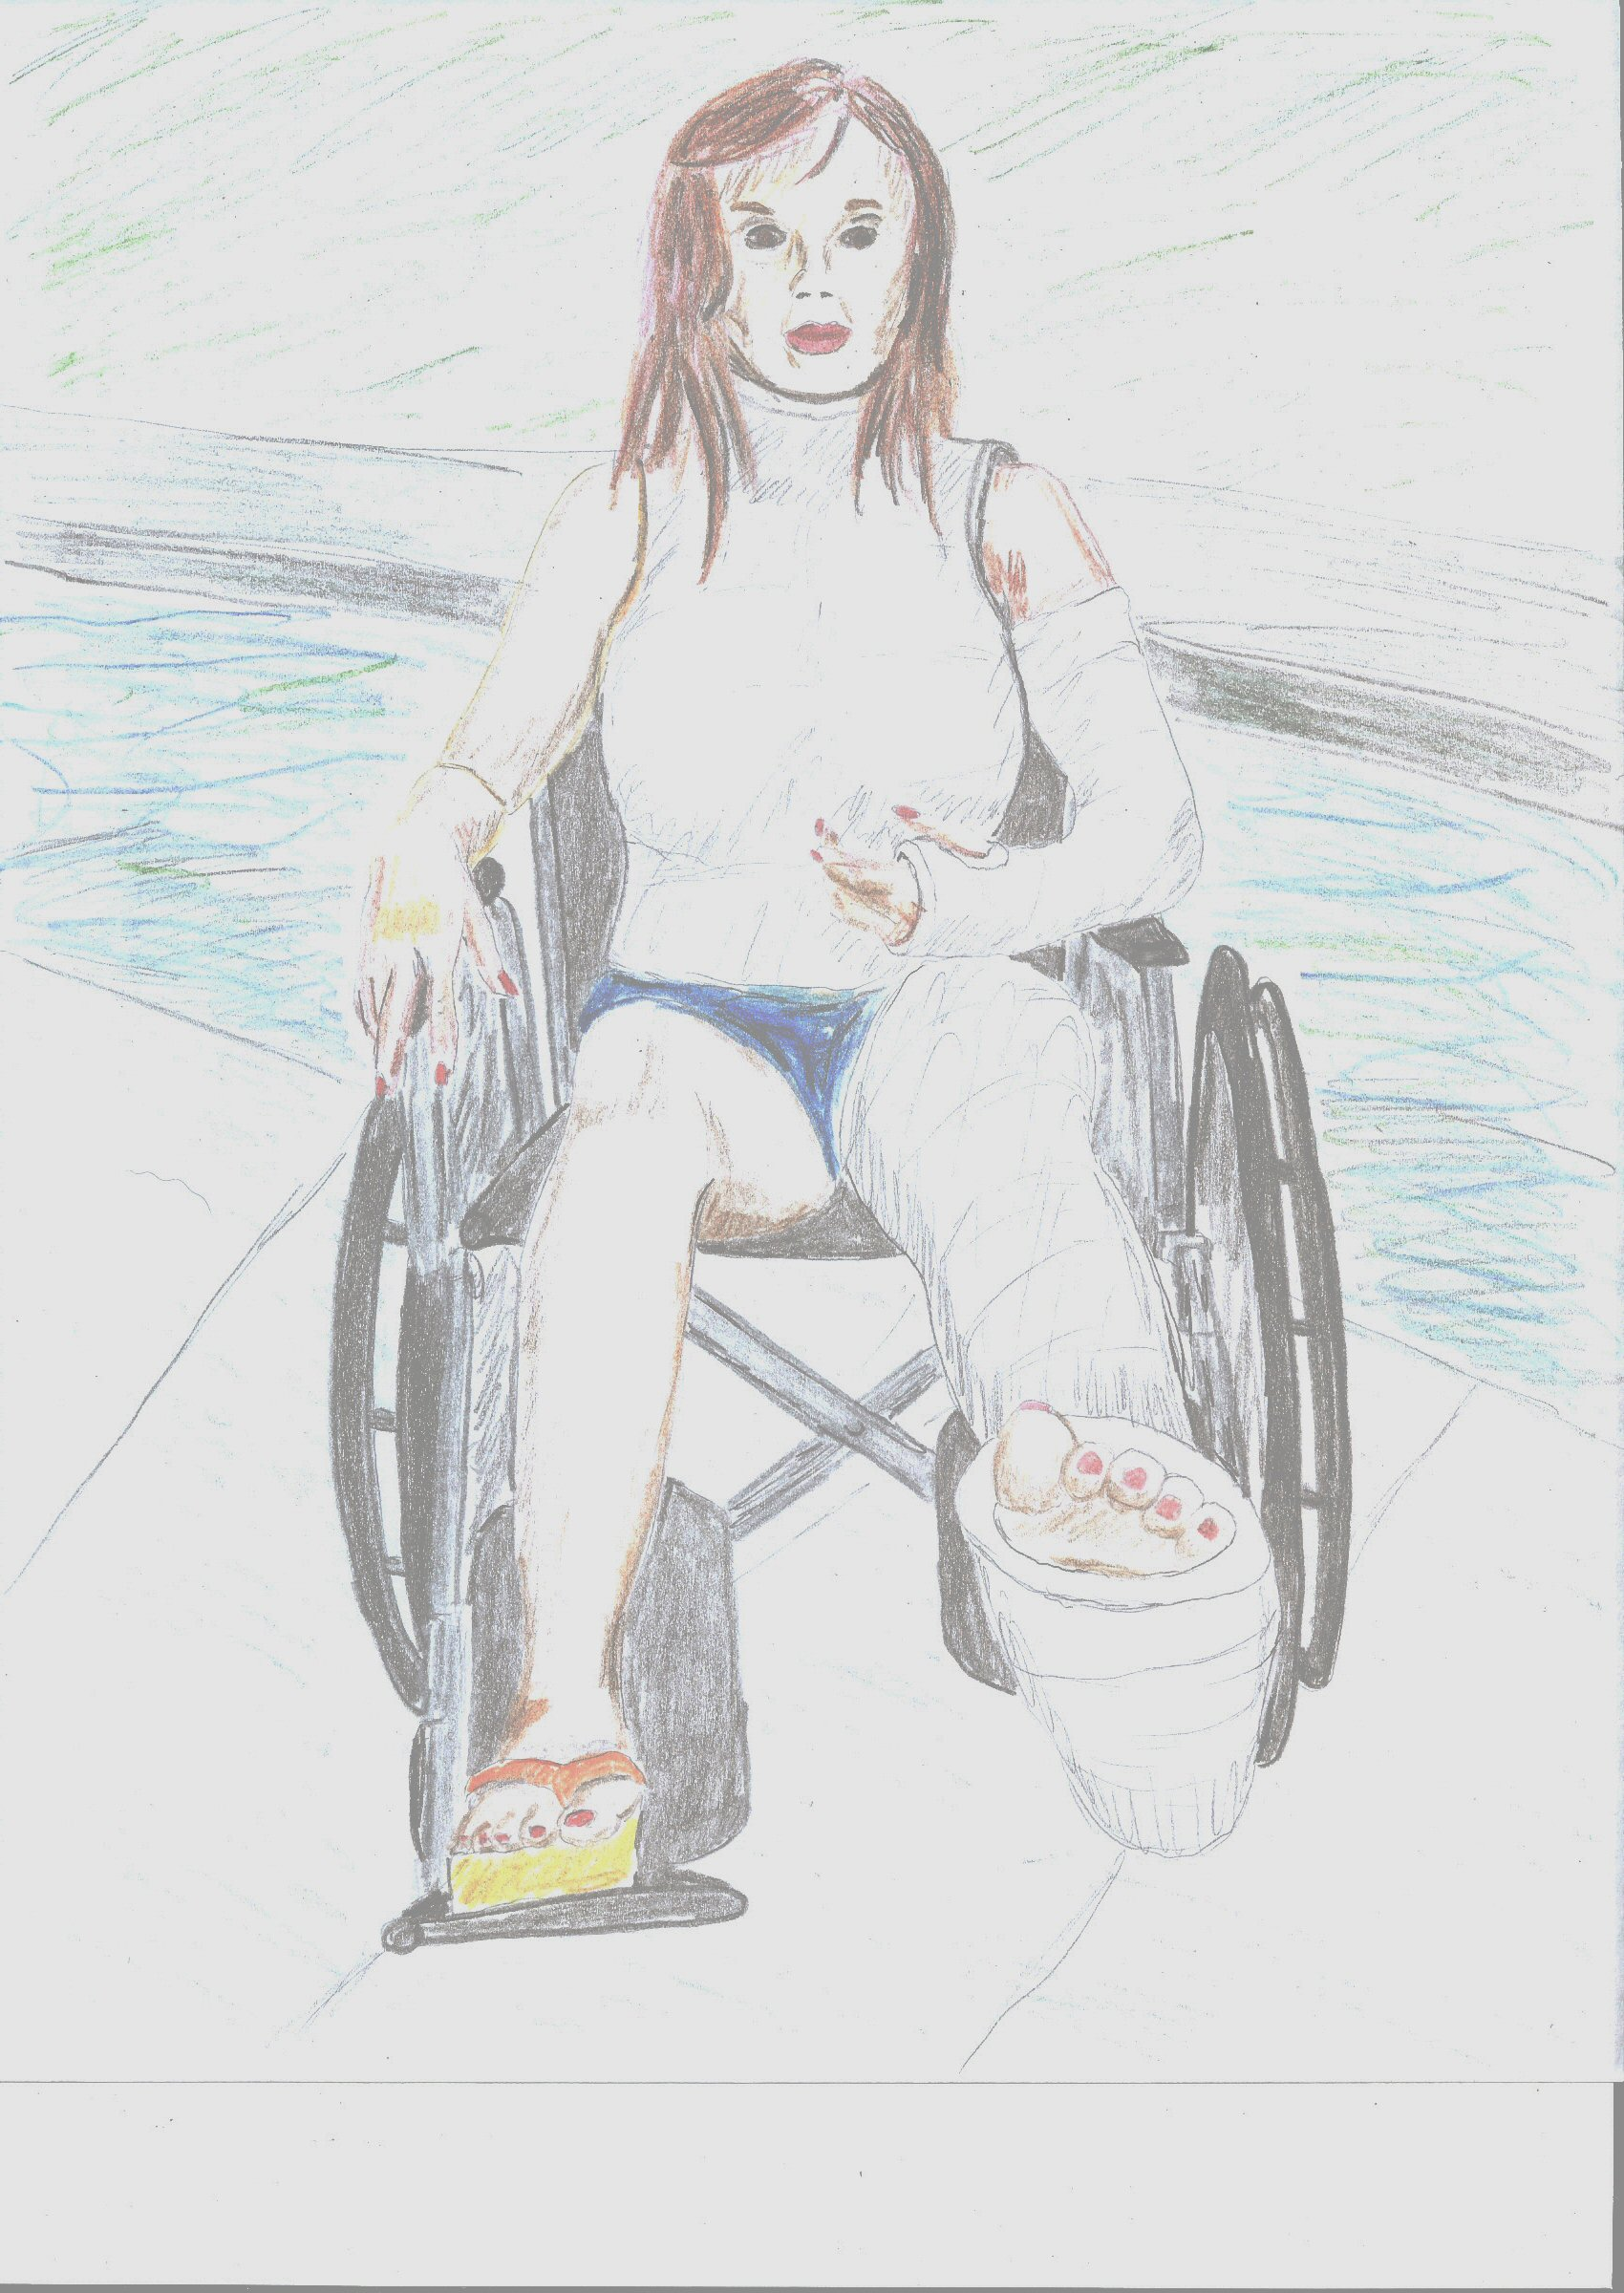
\includegraphics[width=\textwidth]{images/kicks39a.jpg}
\end{center}

\newpage
\begin{center}
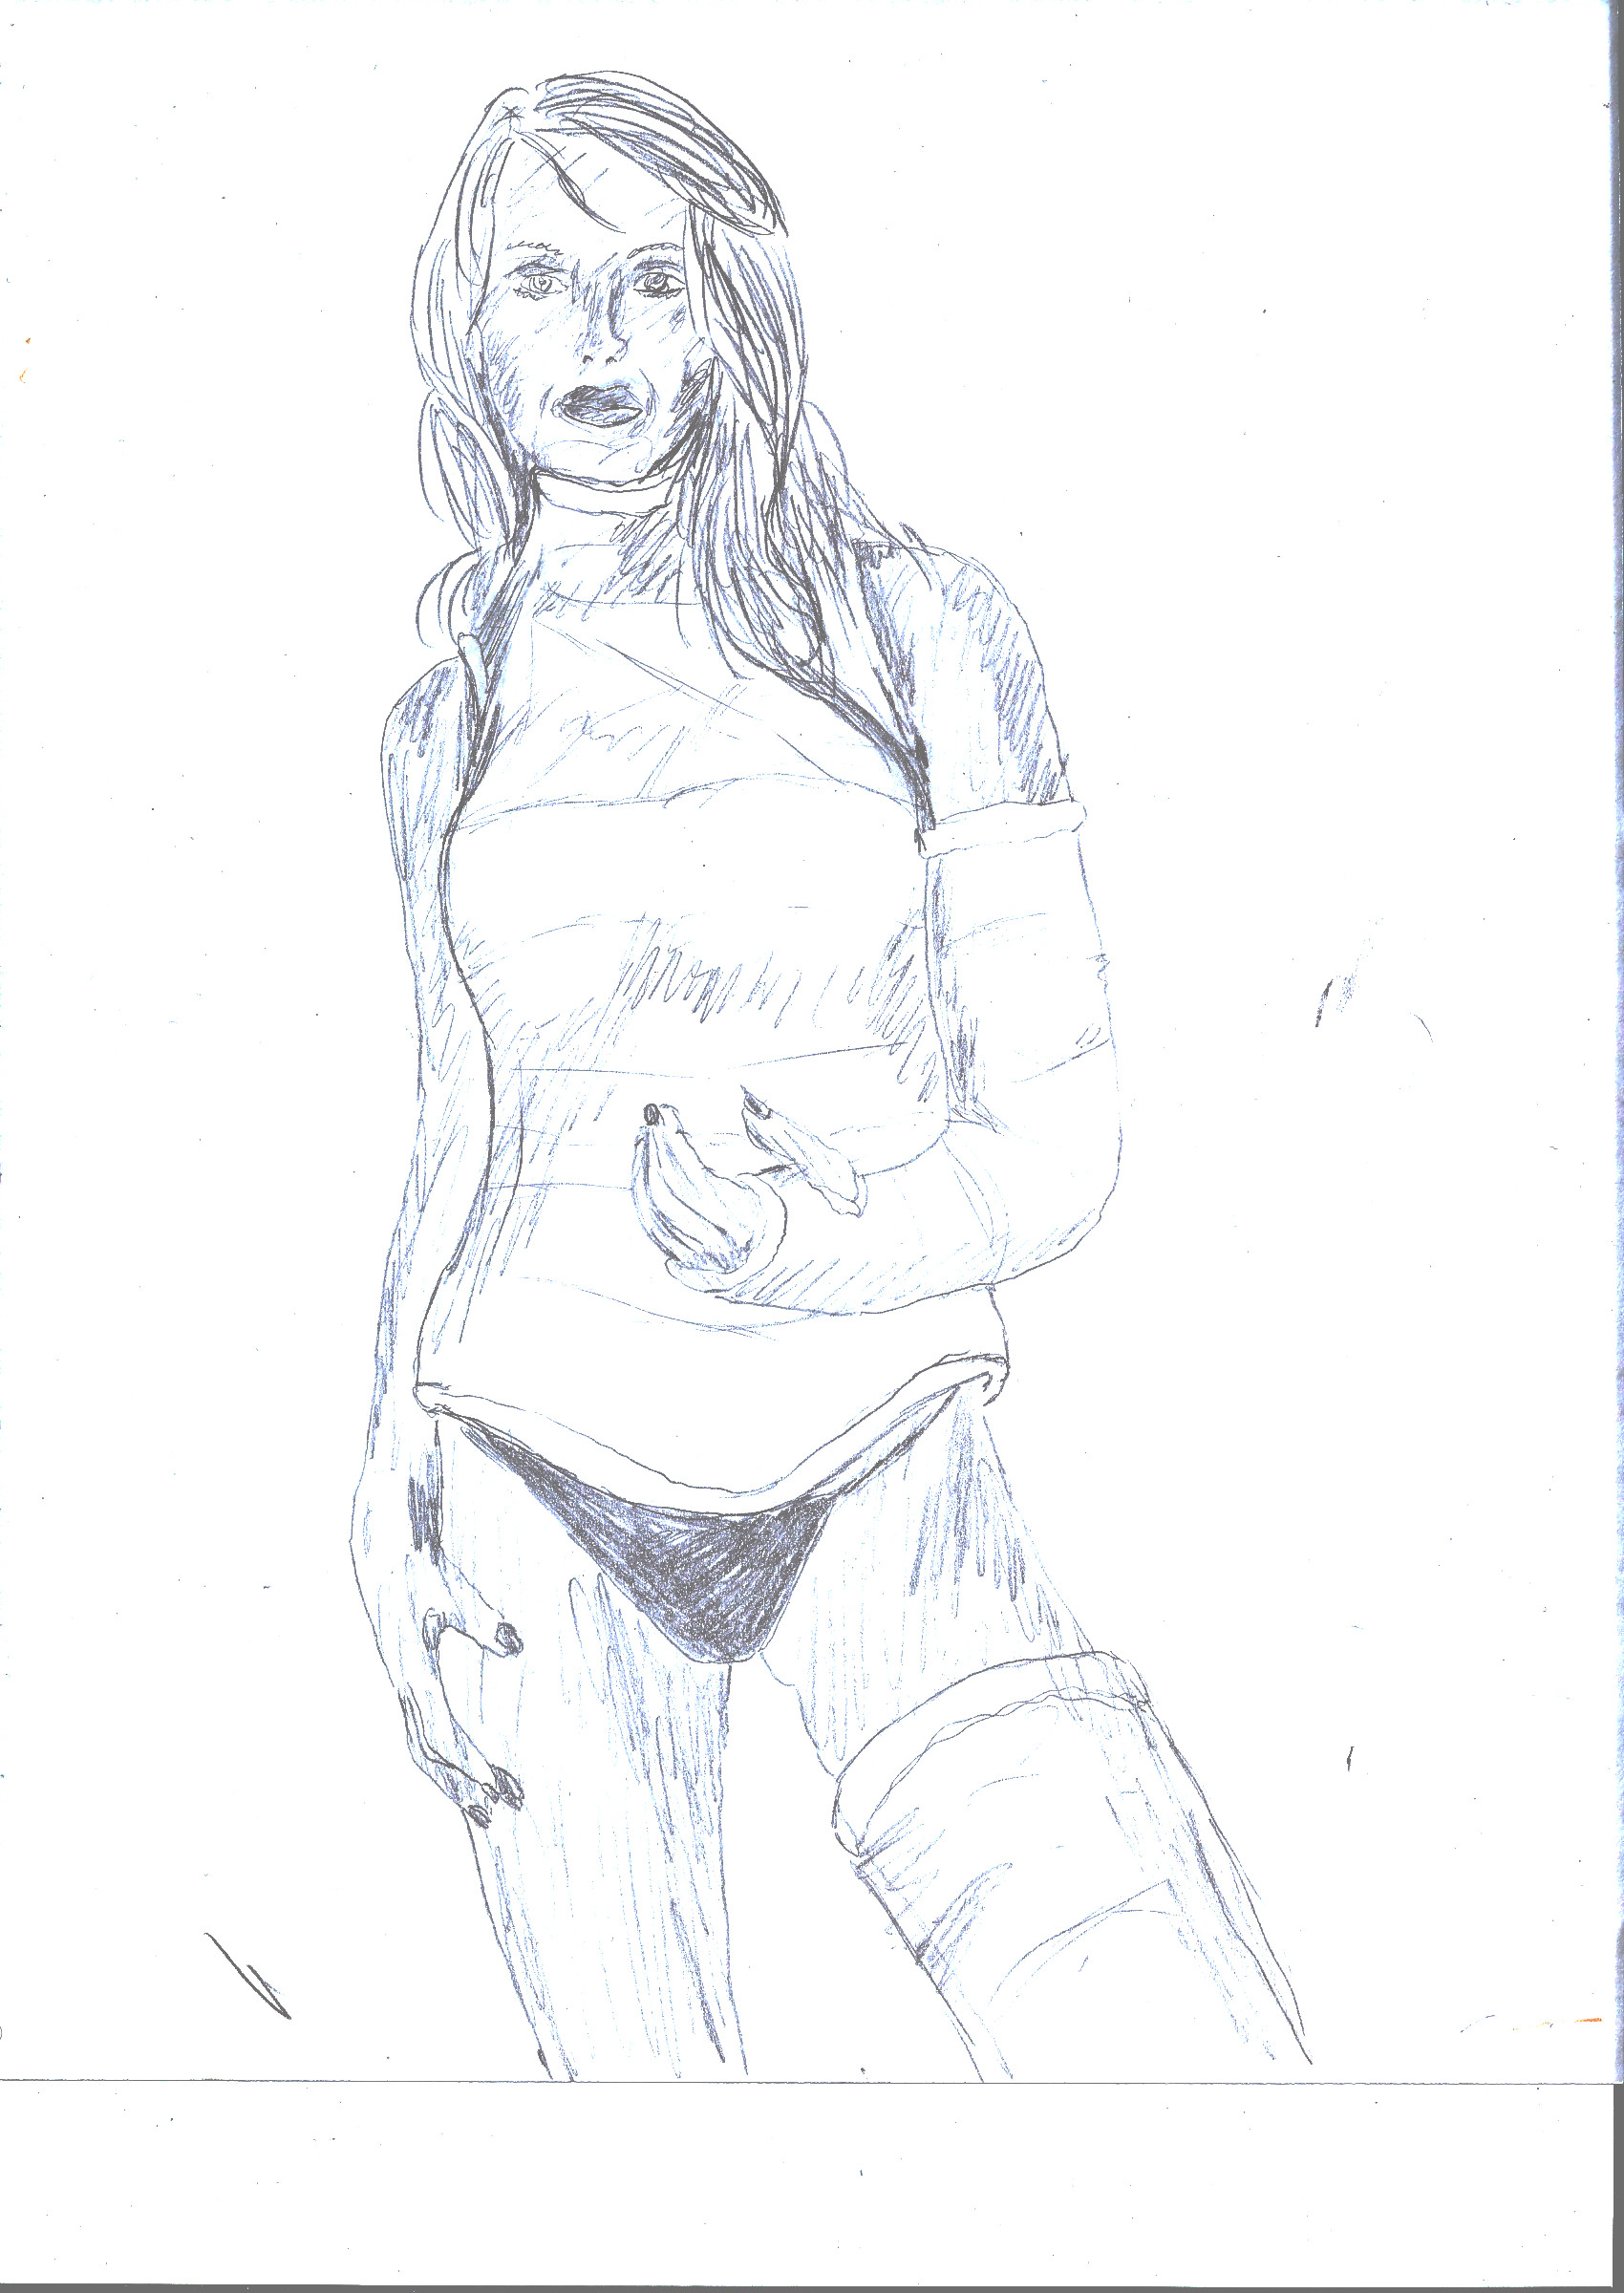
\includegraphics[width=\textwidth]{images/kicks39b.jpg}
\end{center}
